\section{Background and introduction}\label{sec:Intro}

Many, if not all, galactic nuclei have harboured a massive black hole (MBH) during their evolution \citep{Lynden-Bell1971, Soltan1982, Rees1984}. Observations have shown that there exist well-defined correlations between the MBHs' masses and the properties of their host galaxies, such as bulge luminosity, mass, velocity dispersion and light concentration \citep{Kormendy1995, Magorrian1998, Ferrarese2000, Gebhardt2000, Graham2001, Tremaine2002, Marconi2003, Haring2004, Graham2007, Graham2011}. These suggest coeval evolution of the MBH and galaxy \citep{Peng2007, Jahnke2011}, possibly with feedback mechanisms coupling the two \citep{Haiman2004, Volonteri2009}. The MBH and the surrounding spheroidal component share a common history, such that the growth of one can inform us about the growth of the other.

The best opportunity to study MBHs comes from the compact object in our own galactic centre (GC), which is coincident with Sagittarius A* (Sgr A*). Through careful monitoring of stars orbiting the GC, this has been identified as an MBH of mass $M_\bullet = 4.31 \times 10^6 M_\odot$ at a distance of only $R_0 = 8.33\units{kpc}$ \citep{Gillessen2009}.

According to the no-hair theorem, the MBH should be described completely by just its mass $M_\bullet$ and spin $a$, since we expect the charge of an astrophysical black hole to be negligible \citep{Israel1967, Israel1968, Carter1971, Hawking1972, Robinson1975, Chandrasekhar1998}. The spin parameter $a$ is related to the BH's angular momentum $J$ by
\begin{equation}
J = M_\bullet ac;
\end{equation}
it is often convenient to use the dimensionless spin
\begin{equation}
a_\ast = \frac{cJ}{GM_\bullet^2}.
\end{equation}
As we have a good estimate of the mass, to gain a complete description of the MBH we have only to measure its spin; this shall give us insight into its history and role in the evolution of the Galaxy.

The spin of an MBH is determined by several competing processes. An MBH accumulates mass and angular momentum through accretion \citep{Volonteri2010}. Accretion from a gaseous disc shall spin up the MBH, potentially leading to high spin values \citep{Volonteri2005}, while a series of randomly orientated accretion events leads to a low spin value: we expect an average value $|a_\ast| \sim 0.1$--$0.3$ \citep{King2006, King2008}. The MBH also grows through mergers \citep{Yu2002, Malbon2007}. Minor mergers with smaller black holes (BHs) can decrease the spin \citep{Hughes2003, Gammie2004}, while a series of major mergers, between similar mass MBHs, would lead to a likely spin of $|a_\ast| \sim 0.69$ \citep{Berti2008, Berti2007, Gonzalez2007}. Measuring the spin of MBHs shall help us understand the relative importance of these processes, and perhaps gain a glimpse into their host galaxies' pasts.

Elliptical and spiral galaxies are believed to host MBHs of differing spins because of their different evolutions: we expect MBHs in elliptical galaxies to have on average higher spins than black holes in spiral galaxies, where random, small accretion episodes have played a more important role \citep{Volonteri2007, Sikora2007}.

It has been suggested that the spin of the Galaxy's MBH could be inferred from careful observation of the orbits of stars within a few milliparsecs of the GC \citep{Merritt2010}, although this is complicated because of perturbations due to other stars, or from observations of quasi-periodic oscillations in the luminosity of flares believed to originate from material orbiting close to the innermost stable orbits \citep{Genzel2003a, Belanger2006, Trippe2007, Hamaus2009, Kato2010}, though there are difficulties in interpreting these results \citep{Psaltis2008a}.

%This latter method, combined with a disc-seismology model, has produced a value of the dimensionless spin of $a_\ast = 0.44 \pm 0.08$. To obtain this result \citet{Kato2010} have combined their observations of Sgr A* with observations of galactic X-ray sources containing solar mass BHs, to find a best-fit unique spin parameter for all BHs. However, it is not clear that all BHs should share the same value of the spin parameter; especially considering that the BHs considered here differ in mass by six orders of magnitude, with none in the intermediate range. Even if BH spin is determined by a universal process, we still expect some distribution of spin parameters \citep{King2008, Berti2008}. Thus we cannot precisely determine the spin of the galactic centre's MBH from an average including other BHs.

The spins of MBHs in active galactic nuclei have been inferred using X-ray observations of $\mathrm{Fe}$ $\mathrm{K}$ emission lines \citep{Miller2007, McClintock2011}. So far this has been done for a handful of other galaxies' central MBHs \citep{Brenneman2006, Miniutti2009, Schmoll2009, delaCallePerez2010, Zoghbi2010, Nardini2011,  Patrick2011}. Estimates for the spin cover a range of values up to the maximal value for an extremal Kerr black hole. Typical values are in the intermediate range of $a_\ast \sim 0.7$ with an uncertainty of about $10\%$ on each measurement.

While we can use the spin of other BHs as a prior, to inform us of what we should expect to measure for the spin of the Galaxy's MBH, it is desirable to have an independent observation, a direct measurement.

An exciting means of inferring information about the MBH is through gravitational waves (GWs) emitted when compact objects (COs), such as stellar mass BHs, neutron stars (NSs), white dwarfs (WDs) or low mass main sequence (MS) stars, pass close by \citep{Sathyaprakash2009}. A space-borne detector, such as the Laser Interferometer Space Antenna (LISA) or the evolved Laser Interferometer Space Antenna (eLISA), is designed to be able to detect GWs in the frequency range of interest for these encounters \citep{Bender1998, Danzmann2003, Jennrich2011, Amaro-Seoane2012a}. The identification of waves requires a set of accurate waveform templates covering parameter space. Much work has already been done on the waveforms generated when companion objects inspiral towards an MBH \citep{Glampedakis2005, Barack2009}; as they orbit, the GWs carry away energy and angular momentum, causing the orbit to shrink until eventually the object plunges into the MBH. These systems are typically formed following two-body encounters so the initial orbits are highly eccentric; a burst of radiation is emitted during each periapse passage. These are extreme mass-ratio bursts (EMRBs; \citealt*{Rubbo2006}). Assuming that the companion is not scattered from its orbit, and does not plunge straight into the MBH, its orbit evolves, becoming more circular, and it shall begin to continuously emit significant gravitational radiation in the LISA/eLISA frequency range. The resulting signals are extreme mass-ratio inspirals (EMRIs; \citealt{Amaro-Seoane2007}).

Studies of these systems have usually focused upon the phase when the orbit is close to plunge and completes a large number of cycles in the detector's frequency band, allowing a high signal-to-noise ratio (SNR) to be accumulated. Here, we investigate high eccentricity orbits. These are the initial bursting orbits from which an EMRI may evolve. The event rate for the detection of such EMRBs with LISA has been estimated to be as high as $15\units{yr^{-1}}$ \citep{Rubbo2006}, although this has been subsequently revised downwards to the order of $1\units{yr^{-1}}$ \citep{Hopman2007}. Even if only a single burst is detected during a mission, this is still an exciting possibility since the information carried by the GW should give an unparalleled probe of the structure of spacetime of the GC. Exactly what can be inferred depends upon the orbit, which we begin to investigate here. 

We make the simplifying assumption that all these orbits are marginally bound, or parabolic, since highly eccentric orbits appear almost indistinguishable from an appropriate parabolic orbit. Here ``parabolic'' and ``eccentricity'' refer to the energy of the geodesic and not to the geometric shape of the orbit.\footnote{Marginally bound Keplerian orbits in flat spacetime are parabolic in both senses.} Following such a trajectory an object may make just one pass of the MBH or, if the periapsis distance is small enough, it may complete a number of rotations. Such an orbit is referred to as zoom-whirl \citep{Glampedakis2002a}.

In order to compute the gravitational waveform produced in such a case, we integrate the geodesic equations for a parabolic orbit in Kerr spacetime. We assume that the orbiting body is a test particle, such that it does not influence the underlying spacetime, and that the orbital parameters evolve negligibly during the orbit such that they may be held constant. We use this to construct an approximate numerical kludge (NK) waveform \citep{Babak2007}.

In this dissertation, we create NK waveforms for EMRBs. We begin in \secref{Geodesic} with the construction of the geodesic orbits; these trajectories are used in the construction of NK waveforms as explained in \secref{Kludge}. In \secref{Detector} we establish what the LISA detectors would measure, and in \secref{Signal} how the signal would be analysed. In \secref{Waveforms} we look at our NK waveforms. We give fiducial power-law fits for SNR as a function of periapse radius, which may be of use for back-of-the-envelope estimates. We confirm the accuracy of the kludge waveforms in \secref{Energy} by comparing the energy flux to fluxes calculated using other approaches. The typical error introduced by the NK approximation may be a few percent, but this worsens as the periapsis approaches the last non-plunging orbit.

We may proceed to use the waveforms for parameter estimation. This lies beyond the scope of this work, but demonstrates that EMRBs are useful for inferring the properties of the Galaxy's MBH. 

There are currently no funded space-borne detector missions. The eLISA mission concept remains an active field of study. It is hoped to submit this to the European Space Agency as a potential cornerstone mission. We shall use the classic LISA design for this work. This is done from historical affection in lieu of a definite alternative. When funding for a space-borne detector is secured in the future, it is hoped that it shall have comparable sensitivity to LISA, and that studies using the LISA design shall be a sensible benchmark for comparison. We find that to obtain good results the periapse radius must be $r\sub{p} \lesssim 10 r\sub{g}$, where $r\sub{g} = GM_\bullet / c^2$ is a gravitational radius, at this point the SNR is already high: for parameter estimation the orbit is more important that the signal strength, and so the exact detector performance should be of secondary importance.

Throughout this work we adopt a metric with signature $(+,-,-,-)$. Greek indices are used to represent spacetime indices $\mu = \{0,1,2,3\}$ and lowercase Latin indices from the middle of the alphabet are used for spatial indices $i = \{1,2,3\}$. Uppercase Latin indices from the beginning of the alphabet are used for the output of the two LISA detector-arms $A = \{\mathrm{I}, \mathrm{II}\}$, and lowercase Latin indices from the beginning of the alphabet are used for parameter space. Summation over repeated indices is assumed unless explicitly noted otherwise. Geometric units with $G = c = 1$ are used where noted, but in general factors of $G$ and $c$ are retained.

\section{Parabolic orbits in Kerr spacetime}\label{sec:Geodesic}

\subsection{The metric and geodesic equations}

Astrophysical BHs are described by the Kerr metric \citep{Kerr1963}. In standard Boyer-Lindquist coordinates the line element is (\citealt*{Boyer1967, Hobson2006}, section 13.7)
\begin{equation}
\dd s^2 = \frac{\varrho^2 \Delta}{\Sigma^2}c^2\dd t^2 - \frac{\Sigma \sin^2 \theta}{\varrho^2}\left(\dd \phi - \omega \dd t\right)^2 - \frac{\varrho^2}{\Delta}\dd r^2 - \varrho^2\dd \theta^2,
\end{equation}
where we have introduced functions
\begin{align}
\varrho^2 = {} & r^2 + a^2\cos^2\theta,\\
\Delta = {} & r^2 - \frac{2GM_\bullet r}{c^2} + a^2,\\
\Sigma = {} & \left(r^2 +a^2\right)^2 - a^2\Delta\sin^2\theta,\\
\omega = {} & \frac{2GM_\bullet ar}{c\Sigma}.
\end{align}
For the remainder of this section we shall work in natural units with $G = c = 1$.

Geodesics are parametrized by three conserved quantities (aside from the particle's mass $\mu$): energy (per unit mass) $E$, specific angular momentum about the symmetry axis (the $z$-axis) $L_z$, and Carter constant $Q$ (\citealt{Carter1968, Chandrasekhar1998}, section 62). The geodesic equations are
\begin{align}
\varrho^2 \diff{t}{\tau} = {} & a\left(L_z - aE\sin^2 \theta\right) + \frac{r^2 + a^2}{\Delta}T,\\
\varrho^2 \diff{r}{\tau} = {} & \pm \sqrt{V_r},\\
\varrho^2 \diff{\theta}{\tau} = {} & \pm \sqrt{V_\theta},\\
\varrho^2 \diff{\phi}{\tau} = {} & \frac{L_z}{\sin^2 \theta} - aE + \frac{a}{\Delta}T,
\end{align}
where we have introduced potentials
\begin{align}
T = {} & E\left(r^2 +a^2\right) - aL_z,\\
V_r = {} & T^2 - \Delta\left[r^2 + \left(L_z - aE\right)^2 + Q\right],\\
V_\theta = {} & Q - \cos^2 \theta\left[a^2\left(1 - E^2\right) + \frac{L_z^2}{\sin^2\theta}\right],
\end{align}
and $\tau$ is proper time. The signs of the $r$ and $\theta$ equations may be chosen independently.

For a parabolic orbit $E = 1$; the particle is at rest at infinity. This simplifies the geodesic equations. It also allows us to give a simple interpretation for the Carter constant: this is defined as
\begin{equation}
Q = L_\theta^2 + \cos^2\theta\left[a^2\left(1 - E^2\right) + \frac{L_z^2}{\sin^2\theta}\right],
\end{equation}
where $L_\theta$ is the (non-conserved) specific angular momentum in the $\theta$-direction ($V_\theta = L_\theta^2$). For $E = 1$ we have
\begin{equation}
Q = L_\theta^2 + \cot^2\theta\, L_z^2 = L_\infty^2 - L_z^2;
\end{equation}
here $L_\infty$ is the total specific angular momentum at infinity, where the metric is asymptotically flat \citep{DeFelice1980}.\footnote{See \citet{Rosquist2009} for a discussion of the interpretation of $Q$ in the limit $G \rightarrow 0$, corresponding to a flat spacetime.} This is as in Schwarzschild spacetime.

\subsection{Integration variables and turning points}

In integrating the geodesic equations, difficulties can arise because of the presence of turning points, when the sign of the $r$ or $\theta$ geodesic equation changes. The radial turning points are at the periapsis $r\sub{p}$ and at infinity. We may locate the periapsis by finding the roots of
\begin{align}
V_r = {} & 2M_\bullet r^3 - \left(L_z^2+Q\right)r^2 + 2M_\bullet\left[\left(L_z - a\right)^2 + Q\right]r - a^2 Q = {} 0.
\end{align}
This has three roots, which we shall denote $\{r_1, r_2, r\sub{p}\}$; the periapsis $r\sub{p}$ is the largest real root.\footnote{We do not find the apoapsis as a (fourth) root to this equation as we have removed it by taking $E = 1$ before solving. This turning point can be found by setting the unconstrained expression for $V_r$ equal to zero, and then solving for $E(r)$; taking the limit $r \rightarrow \infty$ gives $E \rightarrow 1$ \citep{Wilkins1972}.}

We avoid the difficulties associated with the turning point by introducing an angular variable that always increases with proper time \citep{Drasco2004}: inspired by Keplerian orbits, we parametrize our trajectory by
\begin{equation}
r = \frac{p}{1+e\cos\psi},
\end{equation}
where $e = 1$ is the eccentricity and $p = 2r\sub{p}$ is the semilatus rectum. As $\psi$ covers its full range from $-\pi$ to $\pi$, $r$ traces out one complete orbit from infinity through the periapsis at $\psi = 0$ back to infinity. The geodesic equation for $\psi$ is
\begin{align}
\varrho^2 \diff{\psi}{\tau} = {} & \left\{M_\bullet\left[2r\sub{p} - \left(r_1 + r_2\right)\left(1 + \cos\psi\right) \vphantom{\frac{r_1 r_2}{2r\sub{p}}} \right.\right. \nonumber \\*
 {} & + \left.\left. \frac{r_1 r_2}{2r\sub{p}}\left(1 + \cos\psi\right)^2\right]\right\}^{1/2}.
\end{align}
This may be integrated without problem. Parametrizing an orbit by its periapsis and eccentricity has the additional benefit of allowing easier comparison with its flat-space equivalent \citep{Gair2005}.

The $\theta$ motion is usually bounded, with $\theta_0 \leq \theta \leq \pi - \theta_0$; in the event that $L_z = 0$ the particle follows a polar orbit and $\theta$ covers its full range \citep{Wilkins1972}. The turning points are given by
\begin{equation}
V_\theta = Q - \cot^2\theta\, L_z^2 = 0.
\end{equation}
If we change variable to $\zeta = \cos^2\theta$, we have a maximum value $\zeta_0 = \cos^2\theta_0$ given by
\begin{equation}
\zeta_0 = \frac{Q}{Q+L_z^2} = \frac{Q}{L_\infty^2}.
\label{eq:theta_0}
\end{equation}
See \figref{L_triangle} for a geometrical visualization.
\begin{figure}
\begin{center}
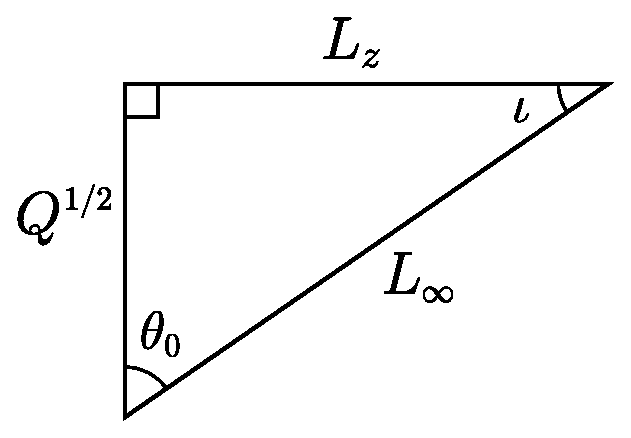
\includegraphics[width=0.3\textwidth]{./images/Triangle.eps}
    \caption{The angular momenta $L_\infty$, $L_z$ and $\sqrt{Q}$ define a right-angled triangle. The acute angles are $\theta_0$, the extremal value of the polar angle, and $\iota$, the orbital inclination \citep{Glampedakis2002}.\label{fig:L_triangle}}
\end{center}
\end{figure}
Let us introduce a second angular variable \citep{Drasco2004}
\begin{equation}
\zeta = \zeta_0\cos^2\chi.
\end{equation}
Over one $2\pi$ period of $\chi$, $\theta$ oscillates from its minimum value to its maximum and back. The geodesic equation for $\chi$ is
\begin{equation}
\varrho^2\diff{\chi}{\tau} = \sqrt{Q + L_z^2},
\end{equation}
and may be integrated simply.

\section{Waveform Construction}\label{sec:Kludge}

For given angular momenta $L_z$ and $Q$, and initial starting position, we can calculate the geodesic trajectory. The orbiting body is assumed to follow this track exactly; we ignore evolution due to the radiation of energy and angular momentum, which should be negligible for EMRBs. From this trajectory we calculate the waveform using a semirelativistic approximation \citep{Ruffini1981}: we assume that the particle moves along a geodesic in the Kerr geometry, but radiates as if it were in flat spacetime. This quick-and-dirty technique is known as a numerical kludge (NK), and has been shown to approximate well results computed by more accurate methods \citep{Babak2007}. It is often compared to a bead travelling along a wire. The shape of the wire is set by the Kerr geodesic, but the bead moves along in flat space.

\subsection{Kludge approximation}

Numerical kludge approximations aim to encapsulate the main characteristics of a waveform by using the exact particle trajectory (ignoring inaccuracies from radiative effects and from the particle's self-force), whilst saving on computational time by using approximate waveform generation techniques.

To start, we build an equivalent flat-space trajectory from the Kerr geodesic. This is done by identifying the Boyer-Lindquist coordinates with a set of flat-space coordinates. We consider two choices here:
\begin{enumerate}
\item Identify the Boyer-Lindquist coordinates with flat-space spherical polars $\{r\sub{BL},$ $\theta\sub{BL},$ $\phi\sub{BL}\} \rightarrow \{r\sub{sph}, \theta\sub{sph}, \phi\sub{sph}\}$, then define flat-space Cartesian coordinates \citep{Gair2005, Babak2007}
\begin{equation}
\boldsymbol{x} = \begin{pmatrix}
r\sub{sph} \sin\theta\sub{sph}\cos\phi\sub{sph} \\
r\sub{sph} \sin\theta\sub{sph}\sin\phi\sub{sph} \\
r\sub{sph} \cos\theta\sub{sph}
\end{pmatrix}.
\end{equation}
\item Identify the Boyer-Lindquist coordinates with flat-space oblate-spheroidal coordinates $\{r\sub{BL}, \theta\sub{BL}, \phi\sub{BL}\} \rightarrow \{r\sub{ob}, \theta\sub{ob}, \phi\sub{ob}\}$ so that the flat-space Cartesian coordinates are
\begin{equation}
\boldsymbol{x} = \begin{pmatrix}
\sqrt{{r\sub{ob}}^2 + a^2} \sin\theta\sub{ob}\cos\phi\sub{ob} \\
\sqrt{{r\sub{ob}}^2 + a^2} \sin\theta\sub{ob}\sin\phi\sub{ob} \\
r\sub{ob} \cos\theta\sub{ob}
\end{pmatrix}.
\end{equation}
These are appealing because in the limit that $G \rightarrow 0$, where the gravitating mass goes to zero, the Kerr metric in Boyer-Lindquist coordinates reduces to the Minkowski metric in oblate-spheroidal coordinates.
\end{enumerate}
In the limit of $a \rightarrow 0$, the two coincide, as they do in the limit of large $r$.

There is no well motivated argument that either coordinate system must yield an accurate GW; their use is justified {\it post facto} by comparison with results obtained from more accurate, and computationally intensive, methods \citep{Gair2005, Babak2007}. The ambiguity in assigning flat-space coordinates reflects the inconsistency of the semirelativistic approximation: the geodesic trajectory was calculated for the Kerr geometry; by moving to flat spacetime we lose the reason for its existence. However, this inconsistency should not be regarded as a major problem; it is just an artifact of the basic assumption that the shape of the trajectory is important for determining the character of the radiation, but the curvature of the spacetime in the vicinity of the source is not. By binding the particle to the exact geodesic, we ensure that the kludge waveform has spectral components at the correct frequencies, but by assuming flat spacetime for generation of GWs they shall not have the correct amplitudes.

\subsection{Quadrupole-octupole formula}

Now we have a flat-space particle trajectory $x\sub{P}^\mu(\tau)$, we may apply a flat-space wave generation formula. We use the quadrupole-octupole formula to calculate the gravitational strain \citep{Bekenstein1973, Press1977, Yunes2008}
\begin{equation}
h^{jk}(t, \boldsymbol{x}) = -\frac{2G}{c^6r}\left(\ddot{I}^{jk} - 2n_i\ddot{S}^{ijk} + n_i\dddot{M}^{ijk}\right)_{t'\, =\, t - r/c},
\label{eq:octupole}
\end{equation}
where an over-dot represents differentiation with respect to time $t$ (and not $\tau$), $t'$ is the retarded time, $r = \left|\boldsymbol{x} - \boldsymbol{x}\sub{P}\right|$ is the radial distance, $\boldsymbol{n}$ is the radial unit vector, and the mass quadrupole ${I}^{jk}$, current quadrupole ${S}^{ijk}$ and mass octupole ${M}^{ijk}$ are defined by
\begin{align}
{I}^{jk}\left(t'\right) = {} & \intd{}{}{{x'}^j{x'}^kT^{00}\left(t', \boldsymbol{x'}\right) }{^3x'};\\
{S}^{ijk}\left(t'\right) = {} & \intd{}{}{{x'}^j{x'}^kT^{0i}\left(t', \boldsymbol{x'}\right)}{^3x'};\\
{M}^{ijk}\left(t'\right)  = {} & \recip{c}\intd{}{}{{x'}^i{x'}^j{x'}^kT^{00}\left(t', \boldsymbol{x'}\right)}{^3x'}.
\end{align}
This is correct for a slowly moving source. It is the familiar quadrupole formula \linebreak[0] (\citealt{Misner1973}, section 36.10; \citealt{Hobson2006}, section 17.9), derived from linearized theory, plus the next order terms. For a point mass, the energy-momentum tensor $T^{\mu\nu}$ contains a $\delta$-function which allows easy evaluation of the integrals of the various moments to give
\begin{align}
{I}^{jk} = {} & c^2\mu x\sub{P}^jx\sub{P}^k;\\
{S}^{ijk} = {} & c\mu v\sub{P}^ix\sub{P}^jx\sub{P}^k;\\
{M}^{ijk} = {} & c\mu x\sub{P}^ix\sub{P}^jx\sub{P}^k.
\end{align}

Since we are only interested in GWs, we use the transverse-traceless (TT) gauge. The waveform is given in the TT gauge by (\citealt{Misner1973}, box 35.1)
\begin{equation}
h\super{TT}_{jk} = P^l_jh_{lm}P^m_k - \recip{2}P_{jk}P^{lm}h_{lm},
\end{equation}
where the (spatial) projection operator $P_{ij}$ is
\begin{equation}
P_{ij} = \delta_{ij} - n_in_j.
\end{equation}

\section{Detection with LISA}\label{sec:Detector}

The classic LISA design is a three arm, space-borne laser interferometer \citep{Bender1998, Danzmann2003}. The three arms form an equilateral triangle that rotates as the system's centre of mass follows a circular, heliocentric orbit, trailing $20^{\circ}$ behind the Earth. eLISA has a similar design, but trails $9^{\circ}$ behind the Earth and only has two arms, which are shorter in length \citep{Jennrich2011}.

To describe the detector configuration, and to transform from the MBH coordinate system to those of the detector, we find it useful to define three coordinate systems: those of the BH at the GC $x_\bullet^i$; ecliptic coordinates centred at the solar system (SS) barycentre $x_\odot^i$, and coordinates that co-rotate with the detector $x\sub{d}^i$. The MBH's coordinate system and the SS coordinate system are depicted in \figref{BH_SS}.
\begin{figure}
\begin{center}
 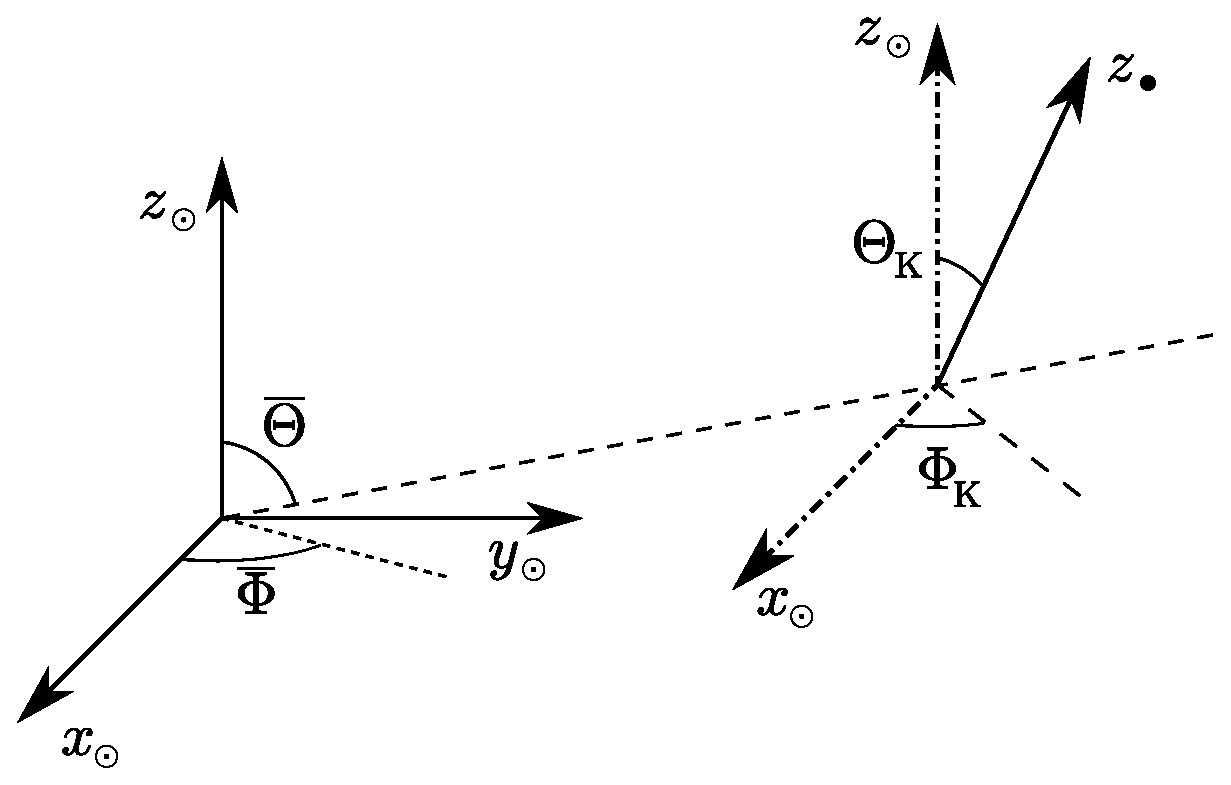
\includegraphics[width=0.5\textwidth]{./images/BH_SS_angles.eps}
    \caption{The relationship between the MBH's coordinate system $x_\bullet^i$ and the SS coordinate system $x_\odot^i$. The MBH's spin axis is aligned with the $z_\bullet$-axis. The orientation of the MBH's $x$- and $y$-axes is arbitrary. We choose $x_\bullet$ to be orthogonal to the direction to the SS.\label{fig:BH_SS}}
\end{center}
\end{figure}
The mission geometry for LISA/eLISA is shown in \figref{SS_LISA}.
\begin{figure}
\begin{center}
 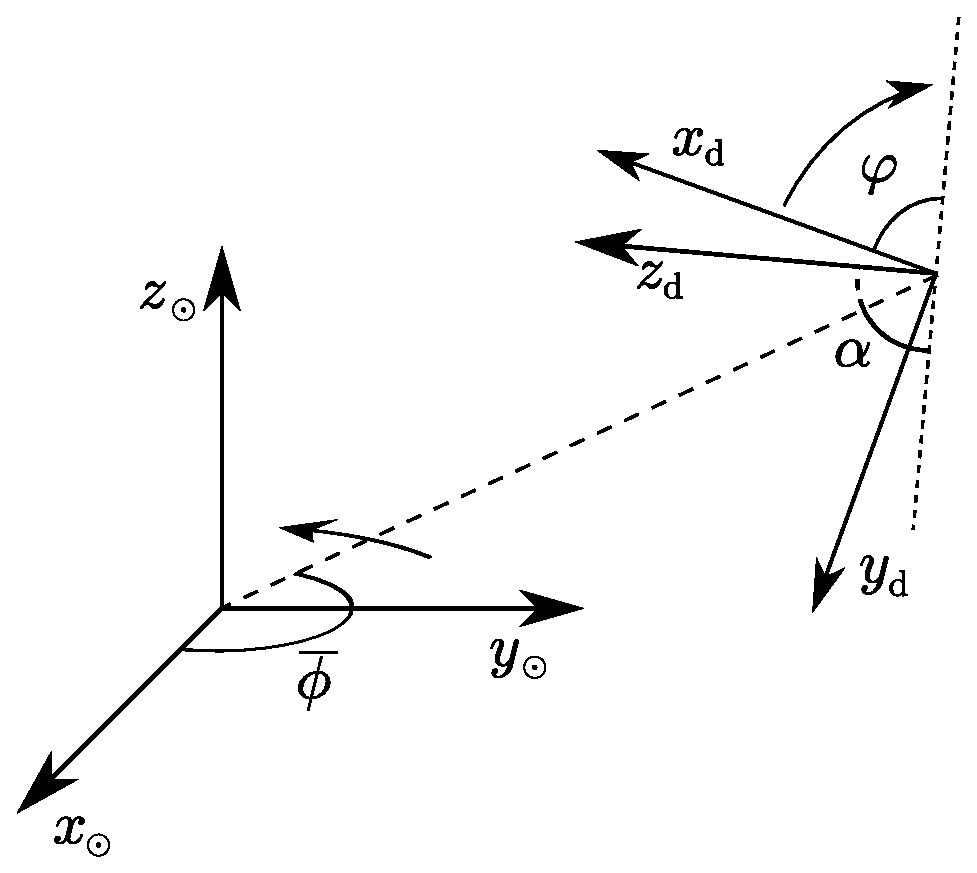
\includegraphics[width=0.4\textwidth]{./images/SS_LISA.eps}
    \caption{The relationship between the detector coordinates $x\sub{d}^i$ and the ecliptic coordinates of the SS $x_\odot^i$ \citep{Bender1998, Jennrich2011}.\label{fig:SS_LISA}}
\end{center}
\end{figure}
We define the detector coordinates such that the detector-arms lie in the $x\sub{d}$-$y\sub{d}$ plane as shown in \figref{LISA_arms}.
\begin{figure}
\begin{center}
 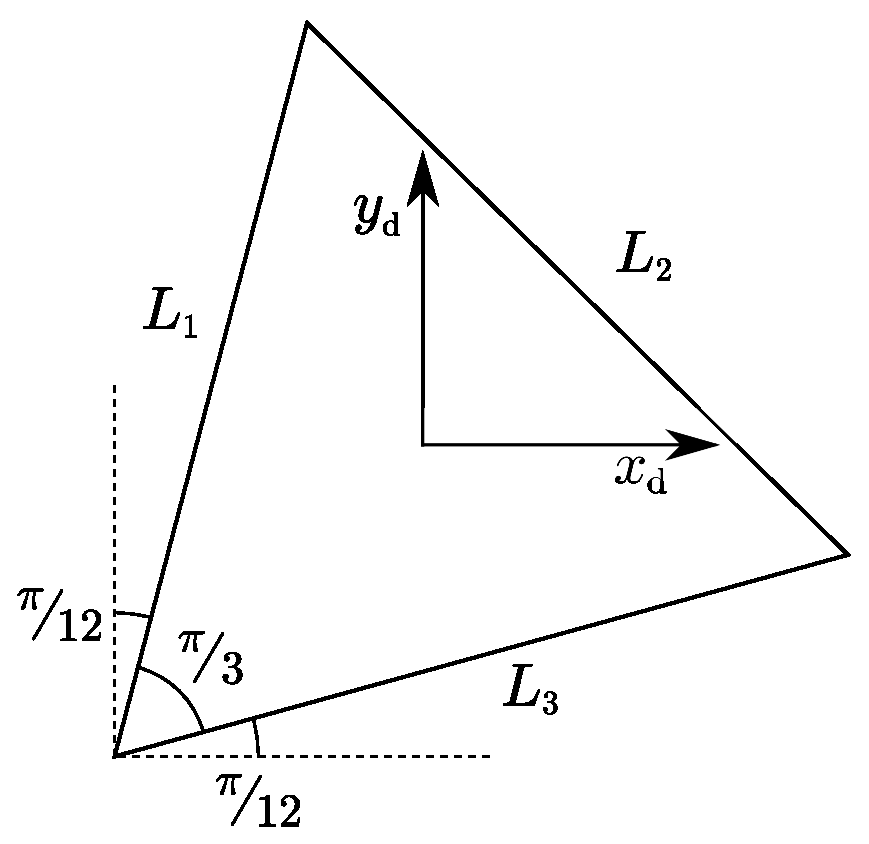
\includegraphics[width=0.32\textwidth]{./images/LISA_arms.eps}
    \caption{The alignment of the three detector arms, with lengths $L_1$, $L_2$ and $L_3$, within the $x\sub{d}$-$y\sub{d}$ plane \citep{Cutler1998}. The origin of the detector coordinates coincides with the centre of mass of the constellation of satellites.\label{fig:LISA_arms}}
\end{center}
\end{figure}
The coordinate systems are related by a series of angles: $\Theta\sub{K}$ and $\Phi\sub{K}$ give the orientation of the MBH's spin axis relative to the SS's coordinates. $\overline{\Theta}$ and $\overline{\Phi}$ give the position of the GC in ecliptic coordinates. $\overline{\phi}$ gives the detector's orbital phase and $\varphi$ gives the rotational phase of the detector arms. Both of these vary linearly with time
\begin{equation}
\overline{\phi}(t) = \omega_\oplus t + \overline{\phi}_0; \quad \varphi(t) = -\omega_\oplus t + \varphi_0;
\end{equation}
where $\omega_\oplus$ corresponds to one rotation per year. Finally, $\alpha = 60^{\circ}$ is the inclination of the detector plane. We have computed the waveforms in the MBH's coordinates, however it is simplest to describe the measured signal using the detector's coordinates.

The strains measured in the three arms can be combined such that LISA behaves as a pair of $90^{\circ}$ interferometers at $45^{\circ}$ to each other, with signals scaled by ${\sqrt{3}}/{2}$ \citep{Cutler1998}. We denote the two detectors as I and II. If we label the change in the three arms' lengths caused by GWs $\delta L_1$, $\delta L_2$ and $\delta L_3$, and use $L$ for the unperturbed length, then detector I measures strain
\begin{equation}
h\sub{I}(t) = \frac{\delta L_1 - \delta L_2}{L} = \frac{\sqrt{3}}{2}\left(\recip{2} h\sub{d}^{xx} - \recip{2}h\sub{d}^{yy}\right),
\end{equation}
and detector II measures
\begin{equation}
h\sub{II}(t) = \frac{\delta L_1 + \delta L_2 - 2 \delta L_3}{\sqrt{3}L} = \frac{\sqrt{3}}{2}\left(\recip{2} h\sub{d}^{xy} + \recip{2} h\sub{d}^{yx}\right).
\end{equation}
We use vector notation $\boldsymbol{h}(t) = \left(h\sub{I}(t), h\sub{II}(t)\right) = \left\{h_A(t)\right\}$ to represent signals from both detectors.

The final consideration for calculating the signal measured by LISA is the time of arrival of the signal: LISA's orbital position changes with time. Fortunately over the timescales of interest for EMRBs, these changes are small. We assume that the position of the SS barycentre relative to the GC is constant: it is defined by the distance $R_0$ and the angles $\overline{\Theta}$ and $\overline{\Phi}$. The time of arrival at the SS barycentre $t_\odot$ is then the retarded time; the time of detection $t\sub{d}$ is
\begin{equation}
t\sub{d} \simeq t_\odot - t\sub{AU}\cos\left[\overline{\phi}(t_\odot) - \overline{\Phi}\right]\sin\overline{\Theta},
\end{equation}
where $t\sub{AU}$ is the light travel-time for the detector's orbital radius. The time $t\sub{d}$ is required for $\phi(t)$ and $\varphi(t)$.

\section{Signal analysis}\label{sec:Signal}

\subsection{Frequency domain formalism}

Having constructed the GW $\boldsymbol{h}(t)$, we may analyse the waveform's properties. We begin with a brief overview of the basic components of signal analysis used for GWs, with application to LISA in particular. This fixes notation. A more complete discussion can be found in \citet{Finn1992} and \citet{Cutler1994}.

The measured strain $\boldsymbol{s}(t)$ is the combination of the signal and the detector noise
\begin{equation}
\boldsymbol{s}(t) = \boldsymbol{h}(t) + \boldsymbol{n}(t);
\end{equation}
we assume that the noise $n_A(t)$ is stationary and Gaussian. It is more convenient to work with the Fourier transform
\begin{equation}
\tilde{g}(f) = \mathscr{F}\{g(t)\} = \intd{-\infty}{\infty}{g(t)e^{2\pi i ft}}{t}.
\end{equation}
For a Gaussian noise signal $n_A(t)$, each Fourier component $\tilde{n}_A(f)$ has a Gaussian probability distribution; the assumption of stationarity means that different Fourier components are uncorrelated, thus \citep{Cutler1994}
\begin{equation}
\left\langle\tilde{n}_A(f)\tilde{n}_B^*(f')\right\rangle_n = \recip{2}\delta(f - f')S_{AB}(f),
\end{equation}
where $\left\langle\ldots\right\rangle_n$ denotes the expectation value over the noise distribution, and $S_{AB}(f)$ is the (single-sided) noise spectral density. For simplicity, we may assume that the noise in the two detectors is uncorrelated, but share the same characterisation so that \citep{Cutler1998}
\begin{equation}
S_{AB}(f) = S_n(f)\delta_{AB}.
\end{equation}

The properties of the noise allow us to define a natural inner product and associated distance on the space of signals \citep{Cutler1994}
\begin{equation}
\innerprod{\boldsymbol{g}}{\boldsymbol{k}} = 2\intd{0}{\infty}{\frac{\tilde{g}_A^\ast(f)\tilde{k}_A(f) + \tilde{g}_A(f)\tilde{k}_A^\ast(f)}{S_n(f)}}{f}.
\label{eq:inner}
\end{equation}
Using this definition, the signal-to-noise ratio is approximately
\begin{equation}
\rho[\boldsymbol{h}] = \innerprod{\boldsymbol{h}}{\boldsymbol{h}}^{1/2}.
\label{eq:SNR}
\end{equation}
The probability of a particular realization of noise $\boldsymbol{n}(t) = \boldsymbol{n}_0(t)$ is
\begin{equation}
p(\boldsymbol{n}(t) = \boldsymbol{n}_0(t)) \propto \exp\left[-\recip{2}\innerprod{\boldsymbol{n}_0}{\boldsymbol{n}_0}\right].
\end{equation}
If the incident waveform is $\boldsymbol{h}(t)$, the probability of measuring signal $\boldsymbol{s}(t)$ is
\begin{equation}
p(\boldsymbol{s}(t)|\boldsymbol{h}(t)) \propto \exp\left[-\recip{2}\innerprod{\boldsymbol{s}-\boldsymbol{h}}{\boldsymbol{s}-\boldsymbol{h}}\right].
\label{eq:sig_prob}
\end{equation}

\subsection{Noise curve}\label{sec:Noise}

LISA's noise has two sources: instrumental noise and confusion noise, primarily from white dwarf binaries. The latter may be divided into contributions from galactic and extragalactic binaries. In this work we use the noise model of \citet{Barack2004}. The shape of the noise curve can be seen in \figref{Noise}. The instrumental noise dominates at both high and low frequencies. The confusion noise is important at intermediate frequencies, and is responsible for the cusp around $10^{-3}\units{Hz}$. eLISA shares the same sources of noise, but is less affected by confusion. Its sensitivity regime is shifted to higher frequencies because of a shorter arm length.
\begin{figure}
\begin{center}
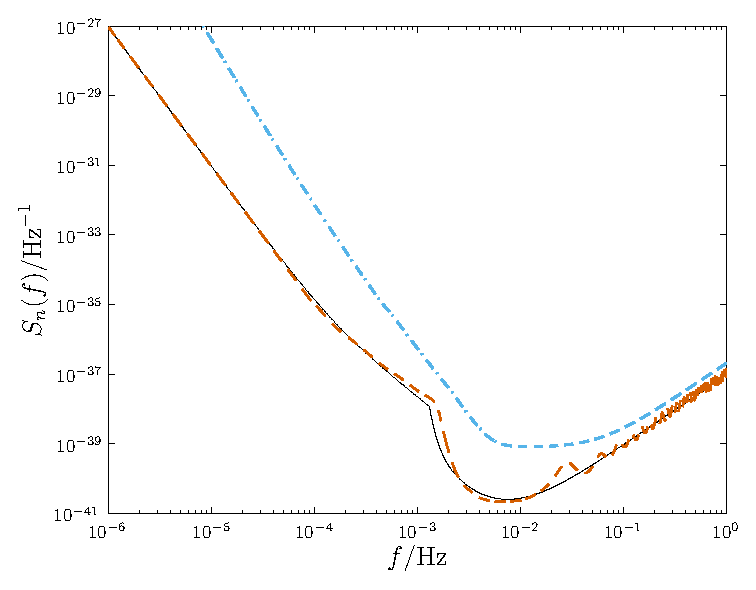
\includegraphics[width=0.6\textwidth]{./images/Fig_Noise}
\caption{The detector noise curves. The solid line indicates the analytic approximation of \citet{Barack2004} used in this work. For comparison, the dashed line is from the online LISA sensitivity curve generator (\url{http://www.srl.caltech.edu/~shane/sensitivity/}; \citealt*{Larson2000, Larson2002}). For bursts from the Galactic Centre we are most interested in the low-frequency region where the two curves are the same. The dot-dashed line shows the eLISA noise curve.\label{fig:Noise}}
\end{center}
\end{figure}

\subsection{Window functions}

There is one remaining complication regarding signal analysis: since we are Fourier transforming a finite signal we encounter spectral leakage; a contribution from large amplitude spectral components leaks into surrounding components (sidelobes), obscuring and distorting the spectrum at these frequencies \citep{Harris1978}. This is an inherent problem with finite signals; it shall be as much of a problem when analysing signals from an actual mission as it is computing waveforms here. To mitigate, but unfortunately not eliminate, these effects, the time-domain signal can be multiplied by a window function. We have adopted the Nuttall four-term window with continuous first derivative \citep{Nuttall1981} for the results presented here.

\section{Waveforms and detectability}\label{sec:Waveforms}

\subsection{Model parameters}

The shape of the waveform depends on a number of parameters: those defining the MBH; those defining the companion object on its orbit, and those defining the LISA detector. Let us define $\boldsymbol{\lambda} = \left\{\lambda^1, \lambda^2, \ldots, \lambda^Z\right\}$ as the set of $Z$ parameters which specify the GW. For our model, the input parameters are:
\begin{enumerate}[leftmargin=*, widest=\:88--88.]
\item[1.] The MBH's mass $M_\bullet$. This is currently well constrained by the observation of stellar orbits about Sgr A* \citep{Ghez2008, Gillessen2009}, with the best estimate being $M_\bullet = (4.31 \pm 0.36) \times 10^6 M_\odot$. This depends upon the galactic centre distance $R_0$ as $M_\bullet = (3.95 \pm 0.06|\sub{stat} \pm 0.18|_{R_0, \, \mathrm{stat}} \pm  0.31|_{R_0, \, \mathrm{sys}}) \times 10^6 M_\odot (R_0 / 8\units{kpc})^{2.19}$, where the errors are statistical, independent of $R_0$; statistical from the determination of $R_0$, and systematic from $R_0$ respectively.
\item[2.] The spin parameter $a_\ast$. Naively this could be anywhere in the range $|a_\ast| < 1$; however it is possible to place an upper bound by contemplating spin-up mechanisms. Considering the torque from radiation emitted by an accretion disc, and swallowed by the BH, it can be shown that $|a_\ast| \lesssim 0.998$ \citep{Thorne1974}. Magnetohydrodynamical simulations of accretion discs produce a smaller maximum value of $|a_\ast| \sim 0.95$ \citep{Gammie2004}. The actual spin value could be much lower than this upper bound depending upon the MBH's evolution (as discussed in \secref{Intro}).
\item[3, 4.] The orientation angles for the black hole spin $\Theta\sub{K}$ and $\Phi\sub{K}$.
\item[5.] The ratio of the SS-GC distance $R_0$ and the CO mass $\mu$, which we denote as $\zeta = R_0/\mu$. This scales the amplitude of the waveform. Bursts, unlike inspirals, do not undergo orbital evolution, hence we cannot break the degeneracy in $R_0$ and $\mu$, and they cannot be inferred separately. The distance, like $M_\bullet$, is constrained by stellar orbits, the best estimate being \citep{Gillessen2009} $R_0 = 8.33 \pm 0.35\units{kpc}$. The mass of the orbiting particle depends upon the type of object: whether it is an MS star, WD, NS or BH. Since we shall not know the $\mu$ precisely, we shall not be able to infer anything more about the distance to the GC.
\item[6, 7.] The angular momentum of the CO. This can be described using either $\{L_z, Q\}$ or $\{L_\infty, \iota\}$. We employ the latter, as the total angular momentum and inclination are less tightly correlated. Assuming spherical symmetry, we expect $\cos \iota$ to be uniformly distributed.
\item[8--10.] A set of coordinates to specify the trajectory. These could be positions at an arbitrary time. We use the angular phases at periapse, $\phi\sub{p}$ and $\chi\sub{p}$ (which determines $\theta\sub{p}$), as well as the time of periapse $t\sub{p}$.
\item[11, 12.] The coordinates of the MBH from the SS barycentre $\overline{\Theta}$ and $\overline{\Phi}$. These may be taken as the coordinates of Sgr A*, as the radio source is expected to be within $20 r\sub{g}$ of the MBH \citep{Reid2003,Doeleman2008}. At the epoch J2000.0 $\overline{\Theta} = {95.607669}^{\circ}$, $\overline{\Phi} = {266.851760}^{\circ}$ \citep{Reid1999, Yusef-Zadeh1999}. They change with time due to the rotation of the SS about the GC; the proper motion is about $6\units{mas\,yr^{-1}}$, mostly in the plane of the galaxy \citep{Reid1999, Backer1999, Reid2003}. The position is already determined to high accuracy: an EMRB can only give weak constraints on source position.\footnote{For comparison, an EMRI, which should be more informative, can only give sky localisation to $\sim 10^{-3}~\mathrm{steradians}$ \citep{Barack2004, Huerta2009}.} Therefore we take it as known and shall not try to infer it.
\item[13, 14.] The orbital position of the LISA satellites given by $\overline{\phi}$ and $\varphi$. We assume that the initial positions are chosen such that $\overline{\phi} = 0$ when $\varphi = 0$ \citep{Cutler1998}; this choice does not qualitatively influence our results. The orbital position should be known, so this need not be inferred.\\
\end{enumerate}
We therefore have a $14$ dimensional parameter space, of which we are interested in inferring $d = 10$ parameters.

\subsection{Waveforms}

\Figref{Examples} shows example waveforms to demonstrate some of the possible variations in the signal. All these assume the standard mass and position for the MBH as well as a $\mu = 10 M_\odot$ orbiting CO; other (randomly chosen) orbital parameters are specified in the captions. Radii are given in terms of the gravitational radius $r\sub{g} = GM_\bullet / c^2$.
\begin{figure}
  \begin{center}
   \subfigure[{Waveform for $a_\ast \simeq 0.12$, $r\sub{p} \simeq 15.6 r\sub{g}$ and $\iota \simeq 2.1$. The SNR for the spherical polar kludge waveform (plotted) is $\rho[\boldsymbol{h}\sub{sph}] \simeq 451$, for the oblate-spheroidal kludge it is $\rho[\boldsymbol{h}\sub{ob}] \simeq 451$ (agreement to $0.01\%$).}]{\label{fig:Orbit_233} 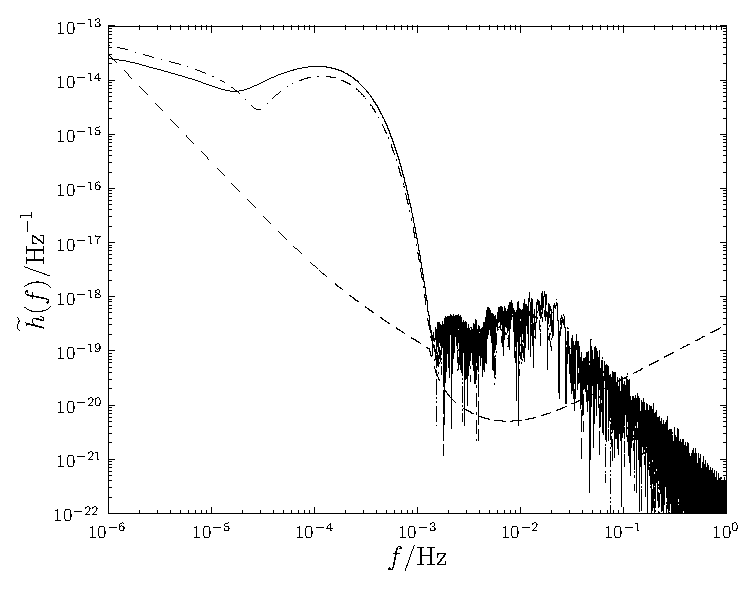
\includegraphics[width=0.47\textwidth]{./images/Fig_new_sph_h_233}} \quad
   \subfigure[{Waveform for $a_\ast \simeq 0.74$, $r\sub{p} \simeq 3.2 r\sub{g}$ and $\iota \simeq 1.2$. The SNR for the spherical polar kludge waveform (plotted) is $\rho[\boldsymbol{h}\sub{sph}] \simeq 70600$, for the oblate-spheroidal kludge it is $\rho[\boldsymbol{h}\sub{ob}] \simeq 74900$.}]{\label{fig:Orbit_135} 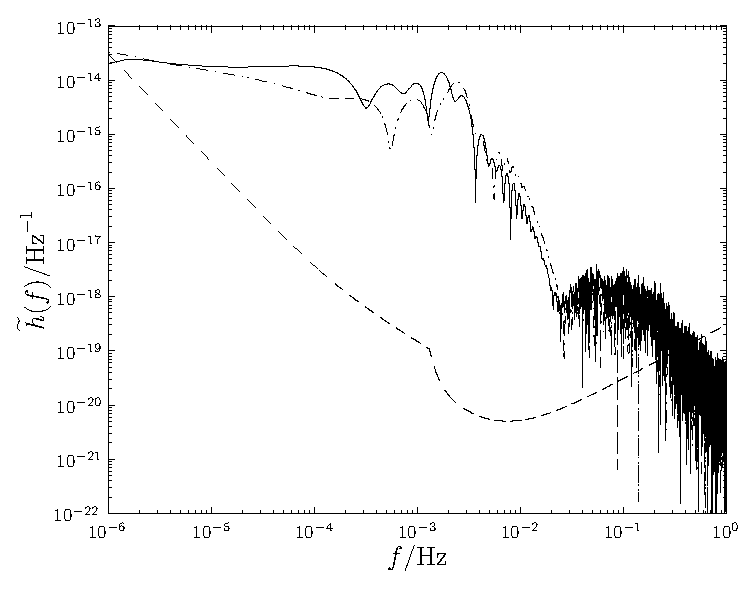
\includegraphics[width=0.47\textwidth]{./images/Fig_new_sph_h_135}}  
\caption{Example burst waveforms from the galactic centre. The strain $\widetilde{h}\sub{I}(f)$ is indicated by the solid line, $\widetilde{h}\sub{II}(f)$ by the dot-dashed line, and the noise curve by the dashed line. The kludge has been formulated using spherical polar coordinates.\label{fig:Examples}}
  \end{center}
\end{figure}

The plotted waveforms use the spherical polar coordinate system for the NK. Using oblate-spheroidal coordinates makes a small difference: on the scale shown here the only discernible difference would be in \figref{Orbit_135}; the maximum difference in the waveform (outside the high-frequency tail) is $\sim 10\%$. In the other cases the difference is entirely negligible (except in the high-frequency tail, which is not of physical significance). This behaviour is typical, for the closest orbits, with the most extreme spin parameters, the maximum difference in the waveforms may be $\sim 30\%$. The difference is largely confined to the higher frequency components, which are most sensitive to the parts of the trajectory closer to the MBH: the change in flat-space radius for the same Boyer-Lindquist radial coordinate causes a slight shift in the shape of the spectrum. Enforcing the same flat-space periapse radius gives worse agreement across the spectrum.

To examine the effect of the coordinate choice, we compare SNRs calculated using the alternative schemes for a selection of orbits. The MBH parameters were fixed as for the GC, the orbital parameters were chosen such that periapse distance was drawn from a logarithmic distribution (down to the innermost stable orbit), and other parameters were drawn from appropriate uniform distributions. The ratio of the two SNRs is shown in \figref{Oblate_sphere}.
\begin{figure}
\begin{center}
 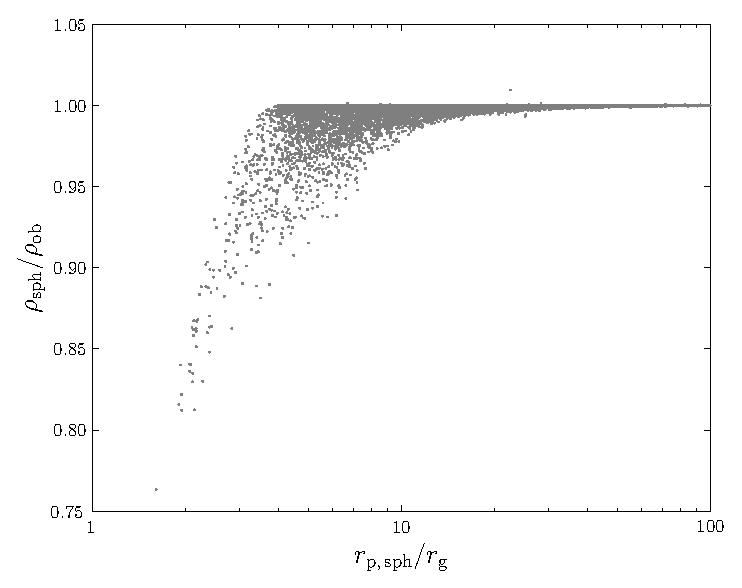
\includegraphics[width=0.6\textwidth]{./images/Fig_SNR_ratio}
 \caption{Ratio of SNR for a waveform calculated using spherical polar coordinates to that for a waveform using oblate-spheroidal coordinates.\label{fig:Oblate_sphere}}
   \end{center}
\end{figure}
The difference from the coordinate systems is only apparent for orbits with very small periapses. There is agreement to $10\%$ down to $r\sub{p} \simeq 4 r\sub{g}$; the maximal difference may be expected to be $\sim 20\%$, this is for periapses that are only obtainable for high spin values.

Since the deviation in the two waveforms is only apparent for small periapses, when the kludge approximation is least applicable, we conclude that the choice of coordinates is unimportant. The potential error of order $10\%$ is no greater than that inherent in the NK approximation (see \secref{Energy}). Without an accurate waveform template to compare against, we do not know if there is a preferable choice of coordinates. We adopt spherical coordinates for easier comparison with existing work.

\subsection{Signal-to-noise ratios}

The detectability of a burst depends upon its SNR. To characterise the variation of $\rho$ we considered a range of orbits. In each case the MBH was assumed to have a mass of $M_\bullet = 4.31 \times 10^6 M_\odot$, to be at the J2000.0 coordinates and a distance of $R_0 = 8.33~\mathrm{kpc}$.

These bursts were calculated for a $1 M_\odot$ CO. From \eqnref{octupole}, the amplitude of the waveform is proportional to the CO mass $\mu$ and so $\rho$ is also proportional to $\mu$; a $10 M_\odot$ object would be ten times louder on the same orbit. To make results mass independent, we shall work in terms of a mass-normalised SNR
\begin{equation}
\hat{\rho}[\boldsymbol{h}] = \left(\frac{\mu}{M_\odot}\right)^{-1}\rho[\boldsymbol{h}].
\end{equation}

The spin of the MBH and the orbital inclination were randomly chosen, and the periapse distance was set so that the distribution would be uniform in log-space (down to the point of the inner-most stable orbit). For each set of these extrinsic parameters, the periapse position, orientation of the MBH, and orbital position of the detector were varied: five random combinations of these intrinsic parameters (each being drawn from a separate uniform distribution) were used for each point.

We take the mean of $\ln \rho$ for each set of randomised intrinsic parameters (starting position, MBH orientation and detector orientation).\footnote{The logarithm is a better quantity to work with since the SNR is a positive-definite quantity that may be distributed over a range of magnitudes \citep[sections 22.1, 23.3]{MacKay2003}. Using median values yields results that are quantitatively similar.}

There exists a correlation between the periapse radius and SNR, as shown in \figref{SNR}.
\begin{figure}
  \begin{center}
  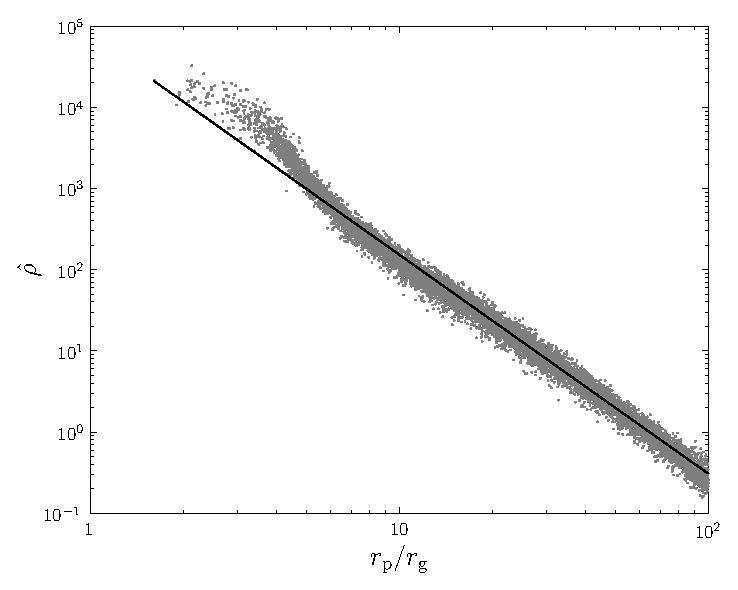
\includegraphics[width=0.6\textwidth]{./images/Fig_SNR}
    \caption{Mass-normalised SNR as a function of periapse radius. The plotted points are the values obtained by averaging over each set of intrinsic parameters. The best fit line is $\log(\hat{\rho}) = -2.69\log(r\sub{p}/r\sub{g}) + 4.88$. This is fitted to orbits with $r\sub{p} >  13.0 r\sub{g}$ and has a reduced chi-squared value of $\chi^2/\nu = 1.73$.\label{fig:SNR}}
  \end{center}
\end{figure}
Closer orbits produce louder bursts. To reflect this relationship, we have fitted a simple fiducial power law, as indicated by the straight line.\footnote{Using oblate-spheroidal coordinates instead of spherical polars gives a fit consistent to within $0.1\%$ as we have excluded the closest orbits.} This was done by maximising the likelihood, assuming that $\ln \rho$ has a Gaussian distribution with standard deviation derived from the scatter because of variation in the intrinsic parameters. The power law appears to be a good fit only for orbits with larger periapses. The shape is predominately determined by the noise curve. The change in the trend reflects the tranisition from approximately power law behaviour to the bucket of the noise curve. Hence, we fit a power law to orbits with a characteristic frequency of $f_\ast = \sqrt{GM_\bullet/r\sub{p}} < 1 \times 10^{-3}\units{Hz}$, so as to avoid spilling over into the bucket. Changing the cut-off within a plausible region alters the fit coefficients by around $0.1$.\footnote{The power law exponent $-2.7$ is inconsistent with $-13/4$ as predicted by the approximate model of \citet{Hopman2007}. This is the result of their approximate waveform model.}

The SNR shows no clear correlation with the other parameters (excluding the mass $\mu$). However, the SNR is sensitive to the intrinsic parameters, in particular the initial position (as this determines the subsequent trajectory), and may vary by an order of magnitude.

Setting a threshold of $\rho = 10$, a $1 M_\odot$ ($10 M_\odot$) object would be expected to be detectable if the periapse distance is less than $27 r\sub{g}$ ($65 r\sub{g}$). \citet{Hopman2007}, assuming a threshold of $\rho = 5$, used an approximate form for the SNR based upon the quadrupole component of a circular orbit; their model, with updated parameters for the MBH, predicts bursts would be detectable out to $66 r\sub{g}$ ($135 r\sub{g}$). We see that this is overly optimistic.

\section{Energy spectra}\label{sec:Energy}

To check that the NK waveforms are sensible, we may compare the energy spectra calculated from these with those obtained from the classic treatment of \citet{Peters1963} and \citet{Peters1964}. This calculates GW emission for Keplerian orbits in flat spacetime, assuming only quadrupole radiation. The spectrum produced should be similar to that obtained from the NK in weak fields, that is for orbits with a large periapsis; however, we do not expect an exact match because of the differing input physics and varying approximations.

In addition to using the energy spectrum, we can also use the total energy flux to check the NK waveforms. The total flux contains less information than the spectrum; however, results have been calculated for parabolic orbits in Schwarzschild spacetime using time-domain black hole perturbation theory \citep{Martel2004}. These should be more accurate than results calculated using the Peters and Mathews formalism.

We do not intend to use the kludge waveforms to calculate an accurate energy flux: this would be inconsistent as we assume that the orbits do not evolve with time. We only calculate the energy flux as a sanity check, to confirm that the kludge approximation is consistent with other approaches.

\subsection{Kludge spectrum}

A gravitational wave in the TT gauge has an effective energy-momentum tensor (\citealt{Misner1973}, section 35.15)
\begin{equation}
T_{\mu\nu} = \frac{c^4}{32\pi G}\left\langle\partial_\mu h_{ij} \partial_\nu h^{ij}\right\rangle,
\end{equation}
where $\langle\ldots\rangle$ indicates averaging over several wavelengths or periods. The flux of energy through a sphere of radius $r = R$ is
\begin{equation}
\diff{E}{t} = \frac{c^3}{32\pi G} R^2 \int{\dd\Omega}\left\langle\diff{h_{ij}}{t}\diff{h^{ij}}{t}\right\rangle,
\end{equation}
with $\int{\dd\Omega}$ representing integration over all solid angles. From \eqnref{octupole} we see that the waves have a $1/{r}$ dependence; if we define
\begin{equation}
h_{ij} = \frac{H_{ij}}{r},
\end{equation}
we see that, using \eqnref{octupole}, the flux is independent of $R$, as required for energy conservation, and
\begin{equation}
\diff{E}{t} = \frac{c^3}{32\pi G} \int{\dd\Omega}\left\langle\diff{H_{ij}}{t}\diff{H^{ij}}{t}\right\rangle.
\end{equation}
If we integrate to find the total energy emitted we obtain
\begin{equation}
E = \frac{c^3}{32\pi G} \int{\dd\Omega}\int_{-\infty}^{\infty}{\dd t} \, \diff{H_{ij}}{t}\diff{H^{ij}}{t}.
\label{eq:integrate_E}
\end{equation}
Since we are considering all time, the localization of the energy is no longer of importance and it is unnecessary to average over several periods. Switching to Fourier representation $\widetilde{H}_{ij}(f) = \mathscr{F}\left\{H_{ij}(t)\right\}$,
\begin{equation}
E = \frac{\pi c^3}{4 G} \int{\dd\Omega}\int_{0}^{\infty}{\dd f} \, f^2 \widetilde{H}^{ij}(f)\widetilde{H}_{ij}^*(f),
\label{eq:total_E}
\end{equation}
using the fact that the signal is real so $\widetilde{H}_{ij}^*(f) = \widetilde{H}_{ij}(-f)$. From this we identify the energy spectrum as
\begin{align}
\diff{E}{f} = \frac{\pi c^3}{4 G} \intd{}{}{}{\Omega} \, f^2 \widetilde{H}^{ij}(f)\widetilde{H}_{ij}^*(f).
\label{eq:NK_dEdf}
\end{align}

\subsection{Peters and Mathews spectrum}

For an orbit of eccentricity $e$ with periapse radius $r\sub{p}$, \citet{Peters1963} give the power radiated into the $n$th harmonic of the orbital angular frequency as
\begin{equation}
P(n) = \frac{32}{5}\frac{G^4}{c^5}\frac{M_\bullet^2\mu^2(M_\bullet + \mu)(1-e)^5}{r\sub{p}^5}g(n,e),
\label{eq:PM_P}
\end{equation}
where the function $g(n,e)$ is defined in terms of Bessel functions of the first kind
\begin{align}
g(n,e) = {} & \frac{n^4}{32}\left\{\left[J_{n-2}(ne) - 2eJ_{n-1}(ne) + \frac{2}{n}J_n(ne) + 2eJ_{n+1}(ne) - J_{n+2}(ne)\right]^2 \right. \nonumber \\*
 & + \left. \left(1 - e^2\right)\left[J_{n-2}(ne) - 2J_n(ne) + J_{n+2}(ne)\right]^2 + \frac{4}{3n^2}\left[J_n(ne)\right]^2\right\}.
% Line breaks follow Peters and Mathews paper
\end{align}
The Keplerian orbital frequency is
\begin{equation}
\omega_1^2 = \frac{G(M_\bullet + \mu)(1 - e)^3}{r\sub{p}^3} = (1 - e)^3\omega\sub{c}^2,
\label{eq:Kepler_freq}
\end{equation}
where $\omega\sub{c}$ is defined as the angular frequency of a circular orbit of radius $r\sub{p}$. The energy radiated per orbit into the $n$th harmonic, that is, at frequency $\omega_n = n\omega_1$, is
\begin{equation}
E(n) = \frac{2\pi}{\omega_1}P(n);
\label{eq:E(n)}
\end{equation}
as $e \rightarrow 1$ for a parabolic orbit, $\omega_1 \rightarrow 0$ as the orbital period becomes infinite. The energy radiated per orbit is then the total energy radiated. The spacing of harmonics is $\Delta\omega = \omega_1$, giving energy spectrum
\begin{equation}
\left.\diff{E}{\omega}\right|_{\omega_n}\omega_1 = E(n).
\end{equation}
Changing to linear frequency $2\pi f = \omega$,
\begin{align}
\left.\diff{E}{f}\right|_{f_n}  = {} & \frac{128\pi^2}{5}\frac{G^3}{c^5}\frac{M_\bullet^2\mu^2}{r\sub{p}^2}(1-e)^2g(n,e) \\*
  = {} & \frac{4\pi^2}{5}\frac{G^3}{c^5}\frac{M_\bullet^2\mu^2}{r\sub{p}^2}\ell(n,e),
\label{eq:PM_spectrum}
\end{align}
where the function $\ell(n,e)$ is defined in the last line. For a parabolic orbit, we must take the limit of $\ell(n,e)$ as $e \rightarrow 1$.

We simplify $\ell(n,e)$ using the recurrence formulae \citep[section 2.12]{Watson1995}
\begin{align}
J_{\nu-1}(z) + J_{\nu+1}(z)  = {} & \frac{2\nu}{z}J_\nu(z)\\*
J_{\nu-1}(z) - J_{\nu+1}(z)  = {} & 2J'_\nu(z),\label{eq:J_derivative}
\end{align}
and eliminate $n$ using
\begin{equation}
n = \frac{\omega_n}{\omega_1} = (1-e)^{-3/2}\tilde{f},
\end{equation}
where $\tilde{f} = \omega_n/\omega\sub{c} = f_n/f\sub{c}$ is a dimensionless frequency. To find the limit we define two new functions
\begin{equation}
A(\tilde{f}) = \lim_{e\rightarrow 1}\left\{\frac{J_n(ne)}{(1-e)^{1/2}}\right\}; \quad B(\tilde{f}) = \lim_{e\rightarrow 1}\left\{\frac{J'_n(ne)}{1-e}\right\}.
\end{equation}
To give a well-defined energy spectrum, both of these must be finite.

The Bessel function has an integral representation
\begin{equation}
J_\nu(z) = \recip{\pi}\intd{0}{\pi}{\cos(\nu\vartheta - z\sin\vartheta)}{\vartheta};
\end{equation}
we want the limit of this for $\nu \rightarrow \infty$, $z \rightarrow \infty$, with $z \leq \nu$. Using the stationary phase approximation, the dominant contribution to the integral comes from the regime in which the argument of the cosine is approximately zero \citep[sections 8.2, 8.43]{Watson1995}:
\begin{align}
J_\nu(z)  \sim {} & \recip{\pi}\intd{0}{\pi}{\cos\left(\nu\vartheta - z\vartheta + \frac{z}{6}\vartheta^3\right)}{\vartheta}\\*
  \sim {} & \recip{\pi}\intd{0}{\infty}{\cos\left(\nu\vartheta - z\vartheta + \frac{z}{6}\vartheta^3\right)}{\vartheta};
\end{align}
this last expression is an Airy integral and has a standard form \citep[section 6.4]{Watson1995}
\begin{equation}
\intd{0}{\infty}{\cos(t^3 + xt)}{t} = \frac{\sqrt{x}}{3}K_{1/3}\left(\frac{2x^{3/2}}{3^{3/2}}\right),
\end{equation}
where $K_\nu(z)$ is a modified Bessel function of the second kind. Using this to evaluate the limit gives
\begin{equation}
J_\nu(z) \sim \recip{\pi}\sqrt{\frac{2(\nu - z)}{3z}}K_{1/3}\left(\frac{2^{3/2}}{3}\sqrt{\frac{(\nu -z)^3}{z}}\right).
\label{eq:J_nu}
\end{equation}
For our case,
\begin{equation}
J_n(ne) \sim \recip{\pi}\sqrt{\frac{2}{3}}(1-e)^{1/2}K_{1/3}\left(\frac{2^{3/2}\tilde{f}}{3}\right),
\end{equation}
and the first limiting function is well defined,
\begin{equation}
A(\tilde{f}) = \recip{\pi}\sqrt{\frac{2}{3}}K_{1/3}\left(\frac{2^{3/2}\tilde{f}}{3}\right).
\end{equation}

To find the derivative we combine \eqnref{J_derivative} and \eqnref{J_nu}, and expand to lowest order yielding
\begin{align}
J'_n(ne) \sim {} & -\frac{1}{2\pi}\sqrt{\frac{2}{3}}(1-e)\left[2^{3/2}K'_{1/3}\left(\frac{2^{3/2}\tilde{f}}{3}\right) + \recip{\tilde{f}}K_{1/3}\left(\frac{2^{3/2}\tilde{f}}{3}\right)\right].
\end{align}
We may re express the derivative using the recurrence formula \citep[section 3.71]{Watson1995}
\begin{equation}
K_{\nu-1}(z) + K_{\nu+1}(z) = -2K'_\nu(z)
\end{equation}
to give
\begin{align}
J'_n(ne)  \sim {} & \frac{1-e}{\sqrt{3}\pi}\left[K_{-2/3}\left(\frac{2^{3/2}\tilde{f}}{3}\right) + K_{4/3}\left(\frac{2^{3/2}\tilde{f}}{3}\right) - \recip{\sqrt{2}\tilde{f}}K_{1/3}\left(\frac{2^{3/2}\tilde{f}}{3}\right)\right].
\end{align}
And so finally we obtain the well-defined
\begin{align}
B(\tilde{f})  = {} & \recip{\sqrt{3}\pi}\left[K_{-2/3}\left(\frac{2^{3/2}\tilde{f}}{3}\right) + K_{4/3}\left(\frac{2^{3/2}\tilde{f}}{3}\right) - \recip{\sqrt{2}\tilde{f}}K_{1/3}\left(\frac{2^{3/2}\tilde{f}}{3}\right)\right].
\end{align}

Having obtained expressions for $A(\tilde{f})$ and $B(\tilde{f})$ in terms of standard functions, we can calculate the energy spectrum for a parabolic orbit. From \eqnref{PM_spectrum}
\begin{equation}
\diff{E}{f} = \frac{4\pi^2}{5}\frac{G^3}{c^5}\frac{M_\bullet^2\mu^2}{r\sub{p}^2}\ell\left(\frac{f}{f\sub{c}}\right),
\label{eq:PM_dEdf}
\end{equation}
where we have used the limit
\begin{align}
\ell(\tilde{f})  = {} & \left[8\tilde{f}^2B(\tilde{f}) - 2\tilde{f}A(\tilde{f})\right]^2 + \left(128\tilde{f}^4 + \frac{4\tilde{f}^2}{3}\right)\left[A(\tilde{f})\right]^2.
\end{align}
This agrees with the $e = 1$ result of \citet{Turner1977}, which was computed by direct integration along unbound orbits. \Figref{ell} shows how $\ell(n,e)$ changes with eccentricity including our result for a parabolic encounter. Although more power is radiated into higher harmonics, the peak of the spectrum does not move much: it is always between $f = f\sub{c}$ and $f = 2 f\sub{c}$, with $f = 2 f\sub{c}$ for $e = 0$ and $f \simeq 1.637 f\sub{c}$ for $e = 1$.
\begin{figure}
\begin{center}
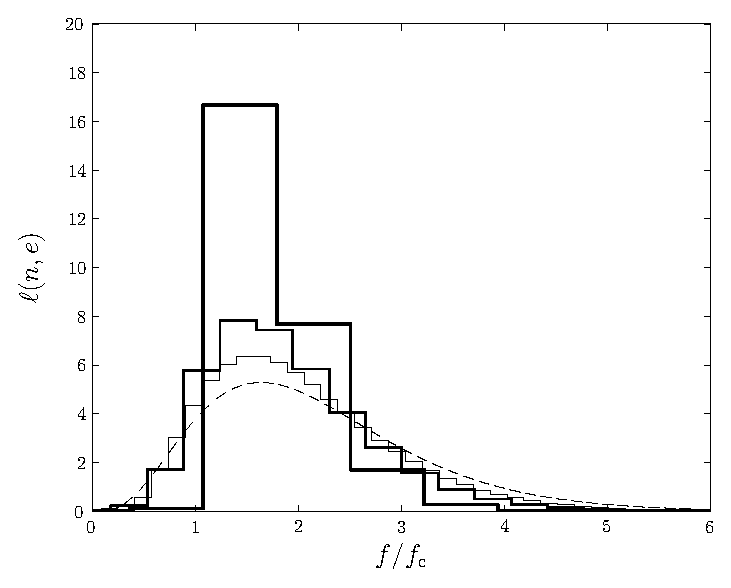
\includegraphics[width=0.6\textwidth]{./images/Fig_ell.eps}
\caption{The relative energy (per orbit) spectrum $\ell(n,e)$ for $e = 0.2$ (heavy line), $e = 0.5$ (medium line), $e = 0.7$ (light line), and the limiting result for $e = 1$ (dashed line) versus frequency. Compare with figure 3 of \citet{Peters1963}.\label{fig:ell}}
\end{center}
\end{figure}

\subsubsection{Total Energy}

To check the validity of this limit we can calculate the total energy radiated by integrating \eqnref{PM_dEdf} over all frequencies, or by summing the energy radiated into each harmonic. These must yield the same result. Summing:
\begin{equation}
E\sub{sum} = \frac{64\pi}{5}\frac{G^3}{c^5}\frac{M_\bullet^2\mu^2}{r\sub{p}^2}\omega\sub{c}(1-e)^{7/2}\sum_n g(n,e),
\end{equation}
where we have used equations \eqnref{PM_P}, \eqnref{Kepler_freq} and \eqnref{E(n)}. \citet{Peters1963} provide the result
\begin{equation}
\sum_n g(n,e) = \frac{1 + (73/24)e^2 + (37/96)e^4}{(1-e^2)^{7/2}}.
\end{equation}
Using this,
\begin{equation}
E\sub{sum} = \frac{64\pi}{5}\frac{G^3}{c^5}\frac{M_\bullet^2\mu^2}{r\sub{p}^2}\omega\sub{c}\frac{1 + (73/24)e^2 + (37/96)e^4}{(1+e)^{7/2}},
\end{equation}
which is perfectly well behaved as $e \rightarrow 1$,
\begin{equation}
E\sub{sum} = \frac{85\pi}{2^{5/2}3}\frac{G^3}{c^5}\frac{M_\bullet^2\mu^2}{r\sub{p}^2}\omega\sub{c}.
\label{eq:PM_total}
\end{equation}
Integrating the energy spectrum \eqnref{PM_dEdf} gives
\begin{equation}
E\sub{int} = \frac{2\pi}{5}\frac{G^3}{c^5}\frac{M_\bullet^2\mu^2}{r\sub{p}^2}\omega\sub{c}\intd{0}{\infty}{\ell(\tilde{f})}{\tilde{f}}.
\end{equation}
The integral can be evaluated numerically as
\begin{equation}
\intd{0}{\infty}{\ell(\tilde{f})}{\tilde{f}} = 12.5216858\ldots = \frac{425}{2^{7/2}3}.
\end{equation}
The two total energies are consistent, $E\sub{int} = E\sub{sum}$.

\subsection{Comparison}

Two energy spectra are plotted in \figref{Energy} for orbits with periapses of $r\sub{p} = 15.0 r\sub{g}$, $30.0 r\sub{g}$ and $60.0 r\sub{g}$.
\begin{figure*}
  \begin{center}
   \subfigure[$r\sub{p} = 15.0 r\sub{g}$, log-log plot.]{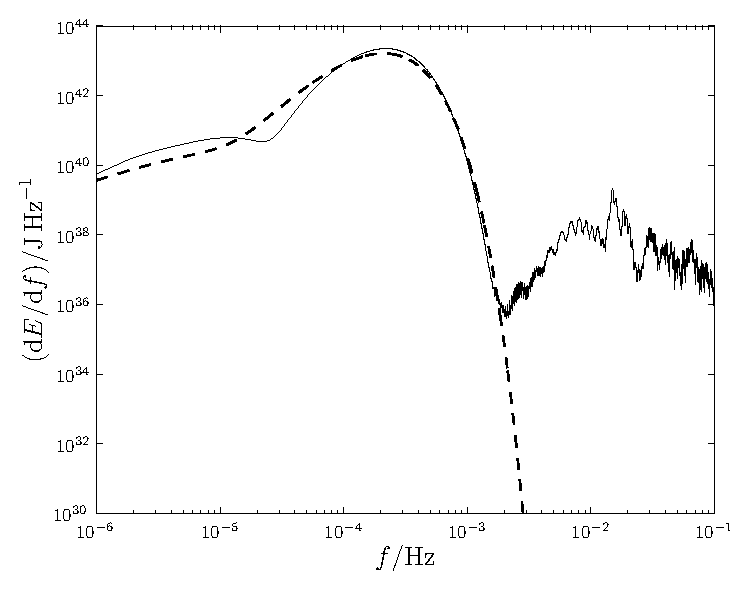
\includegraphics[width=0.47\textwidth]{./images/Fig_Loglog_E_15}} \quad
   \subfigure[$r\sub{p} = 15.0 r\sub{g}$, log-linear plot.]{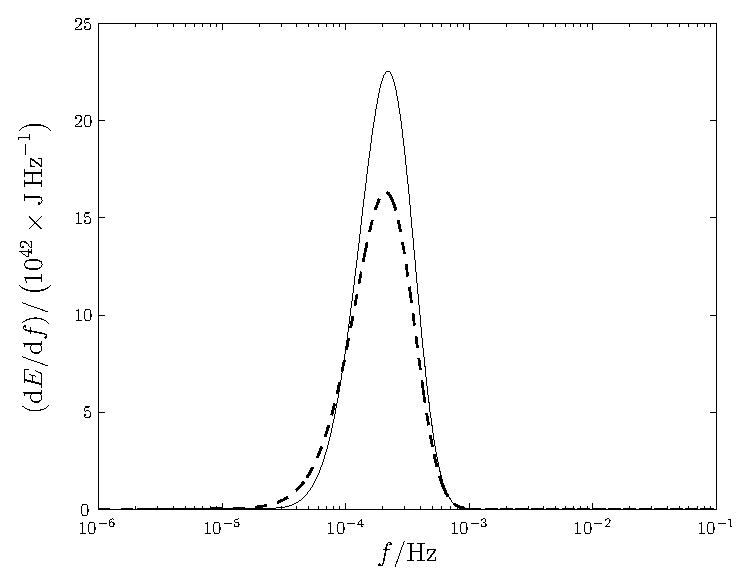
\includegraphics[width=0.47\textwidth]{./images/Fig_Loglin_E_15}} \\
   \subfigure[$r\sub{p} = 30.0 r\sub{g}$, log-log plot.]{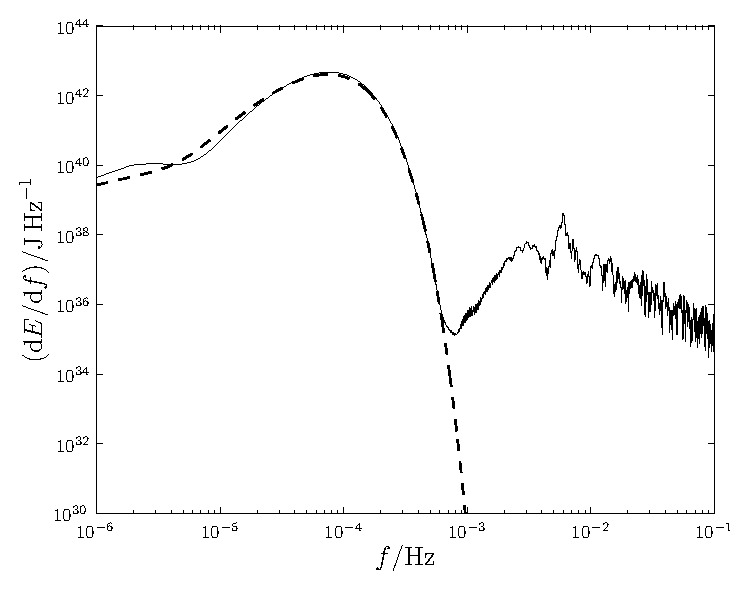
\includegraphics[width=0.47\textwidth]{./images/Fig_Loglog_E_30}} \quad
   \subfigure[$r\sub{p} = 30.0 r\sub{g}$, log-linear plot.]{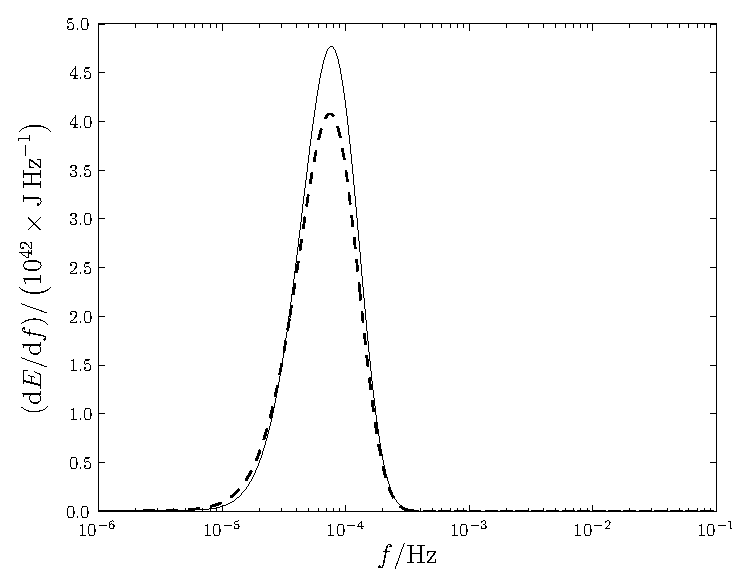
\includegraphics[width=0.47\textwidth]{./images/Fig_Loglin_E_30}} \\
   \subfigure[$r\sub{p} = 60.0 r\sub{g}$, log-log plot.]{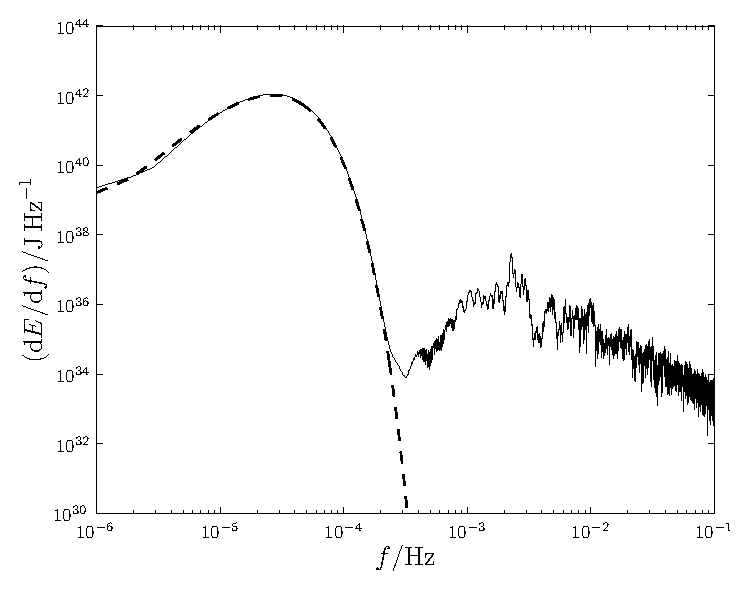
\includegraphics[width=0.47\textwidth]{./images/Fig_Loglog_E_60}} \quad
   \subfigure[$r\sub{p} = 60.0 r\sub{g}$, log-linear plot.]{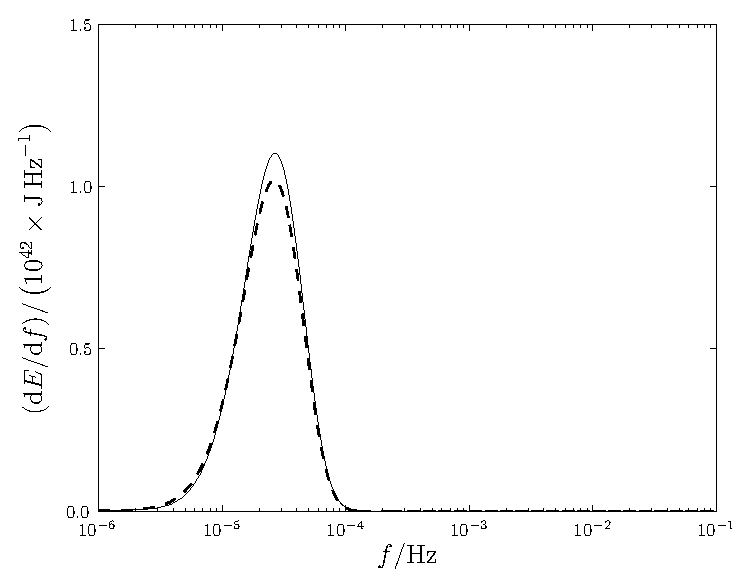
\includegraphics[width=0.47\textwidth]{./images/Fig_Loglin_E_60}}
    \caption{Energy spectra for a parabolic orbit of a $\mu = 10 M_\odot$ object about a Schwarzschild BH with $M_\bullet = 4.31 \times 10^6 M_\odot$. The spectra calculated from the NK waveform is shown by the solid line and the Peters and Mathews flux is indicated by the dashed line. The NK waveform includes octupole contributions. The high frequency tail is the result of spectral leakage.\label{fig:Energy}}
  \end{center}
\end{figure*}
The two spectra appear to be in good agreement, showing the same general shape in the weak-field limit. The NK spectrum is more tightly peaked, but is always within a factor of $2$ at the apex. The peak of the spectrum is shifted to a marginally higher frequency in the NK spectrum primarily because of the addition of the current quadrupole and mass octupole terms.

Comparing the total energy fluxes, ratios of the various energies are plotted in \figref{Energy_ratio}.
\begin{figure*}
  \begin{center}
   \subfigure[Versus periapsis]{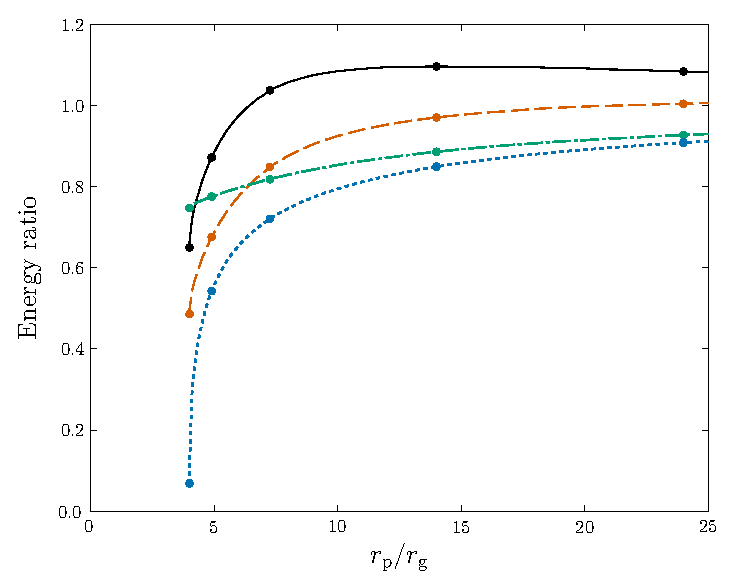
\includegraphics[width=0.48\textwidth]{./images/Fig_Energy_ratio_peri}} \quad
   \subfigure[Versus amount of rotation]{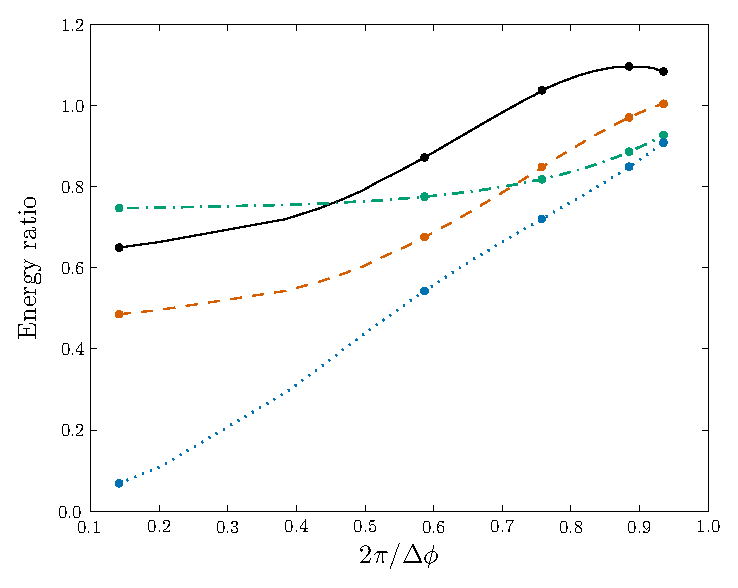
\includegraphics[width=0.48\textwidth]{./images/Fig_Energy_ratio_orbit}}
    \caption{Ratios of energies as a function of periapsis $r\sub{p}$ and $2\pi$ divided by the total angle of rotation in one orbit $\Delta\phi$ ($2\pi/\Delta\phi = 1$ for a Keplerian orbit). The solid line shows the ratio of the numerical kludge and Martel energies $E\sub{NK}/E\sub{M}$; the dashed line shows the ratio of the NK energy calculated using only the mass quadrupole term and the Martel energy $E\sub{NK(Q)}/E\sub{M}$; the dot-dashed line shows the ratio of the quadrupole and quadrupole-octupole NK energies $E\sub{NK(Q)}/E\sub{NK}$, and the dotted line shows the ratio of the Peters and Mathews and quadrupole NK energies $E\sub{PM}/E\sub{NK(Q)}$. The spots show the mapping between the two abscissa scales. Compare with figure 4 of \citet{Gair2005}.\label{fig:Energy_ratio}}
  \end{center}
\end{figure*}
We introduce an additional energy here, the quadrupole NK energy $E\sub{NK(Q)}$. This allows easier comparison with the Peters and Mathews energy which includes only quadrupole radiation. It can be calculated in three ways:
\begin{enumerate}
\item Inserting the waveform $\widetilde{h}(f)$ generated including only the mass quadrupole term in \eqnref{octupole} into \eqnref{total_E} and integrating. This is equivalent to the method used to calculate $E\sub{NK}$.
\item Numerically integrating the quadrupole GW luminosity (\citealt{Misner1973}, section 36.7; \citealt{Hobson2006}, section 18.7)
\begin{equation}
E = \frac{G}{5c^9}\intd{}{}{\dddot{\Ibar}_{ij}\dddot{\Ibar}^{ij}}{t},
\label{eq:E_quad}
\end{equation}
where $\Ibar_{ij} = I_{ij} - (1/3)I\delta_{ij}$ is the reduced mass quadrupole tensor. We can obtain this from \eqnref{integrate_E}, by integrating over all angles when the waveform only contains the mass quadrupole component. This has the advantage of avoiding the effects of spectral leakage or the influence of window functions.
\item Using the analytic expressions for the integral \eqnref{E_quad} given in appendix A of \citet{Gair2005}.
\end{enumerate}
All three agree to within computational error. No difference is visible on the scale plotted in \figref{Energy_ratio}. This demonstrates the validity of the code.

We have used the amount of rotation $\Delta\phi$ as a convenient measure for the abscissa. For an equatorial orbit in Kerr spacetime,
\begin{align}
\Delta\phi  = {} & 2\intd{r\sub{p}}{\infty}{\diff{\phi}{r}}{r} \nonumber \\*
  = {} & \sqrt{\frac{2}{M_\bullet}}L_z\intd{r\sub{p}}{\infty}{\frac{r^2 - 2M_\bullet(1 - a/L_z)r}{(r^2 - 2M_\bullet r + a^2)w}}{r},
\end{align}
where
\begin{equation}
w^2 = r^3 - \frac{L_z^2}{2M_\bullet}r^2 + (L_z - a)^2r;
\end{equation}
$L_z$ is the specific angular momentum about the $z$-axis; $a$ is the spin parameter, and we have adopted units with $G = c = 1$. We shall find it useful to define
\begin{equation}
r_\pm = M_\bullet \pm \sqrt{M_\bullet^2 - a^2},
\end{equation}
and the two nonzero roots of the cubic $w^2$
\begin{equation}
r_{\mathrm{p},\,1} = \frac{L_z^2}{4M_\bullet} \pm \sqrt{\frac{L_z^4}{16M_\bullet^2} - (L_z -a)^2};
\end{equation}
the periapsis is the larger root $r\sub{p} > r_1$. This equation implicitly gives $L_z$ as a function of $r\sub{p}$. The integral may be rewritten as
\begin{equation}
\Delta\phi = \sqrt{\frac{2}{M}}L_z\intd{r\sub{p}}{\infty}{\recip{w}\left(1 + \frac{\alpha_+}{r-r_+} + \frac{\alpha_-}{r-r_-}\right)}{r},
\end{equation}
where
\begin{equation}
\alpha_\pm = \pm\frac{2Mar_\pm - a^2L_z}{2L_z\sqrt{M^2-a^2}}.
\end{equation}
This may be evaluated using elliptic integrals \citep[3.131.8, 3.137.8]{Gradshteyn2000}
\begin{equation}
\Delta\phi = 2 L_z \sqrt{\frac{2}{r\sub{p}M}}\left[\frac{\alpha_+}{r_+}\Pi\left(\frac{r_+}{r\sub{p}}\middle|\frac{r_1}{r\sub{p}}\right) + \frac{\alpha_-}{r_-}\Pi\left(\frac{r_-}{r\sub{p}}\middle|\frac{r_1}{r\sub{p}}\right)\right],
\end{equation}
where $\Pi(n|m) = \int_{0}^{\pi/2}{\dd\vartheta/(1-n\sin^2\vartheta)\sqrt{1-m\sin^2\vartheta}}$ is the complete elliptic integral of the third kind. In the limit of $a \rightarrow 0$ we recover the Schwarzschild result \citep{Cutler1994}
\begin{equation}
\Delta\phi =  2 L_z\sqrt{\frac{2}{r\sub{p}M}}K\left(\frac{r_1}{r\sub{p}}\right),
\end{equation}
where $K(m) = \int_{0}^{\pi/2}{\dd\vartheta/\sqrt{1-m\sin^2\vartheta}}$ is the complete elliptic integral of the first kind.

The ratios all tend towards one in the weak field, as required, but differences become more pronounced in the strong field. The NK energy is larger than the Peters and Mathews result $E\sub{PM}$. This behaviour has been seen before for high eccentricity orbits about a non-spinning BH \citep{Gair2005}. It may be explained by considering the total path length for the different orbits: the Peters and Mathews spectrum assumes a Keplerian orbit, the orbit in Kerr geometry rotates more than this. The greater path length leads to increased emission of gravitational waves and a larger energy flux. Our bead must travel further along its wire. A good proxy for the path length is the angle of rotation $\Delta\phi$; this is $2\pi$ for a Keplerian orbit, in Kerr the angle should be $2\pi$ in the limit of an infinite periapsis, whereas for a periapsis small enough that the orbit shows zoom-whirl behaviour, the total angle may be many times $2\pi$. There is a reasonable correlation between the amount of rotation $2\pi/\Delta\phi$ and the ratio of energies.

Error in the NK energy compared with the time-domain black hole perturbation theory results of Martel comes from two sources: the neglecting of higher order multipole contributions and the ignoring of background curvature. The contribution of the former can be estimated by looking at the difference in the NK energy by including the current quadrupole and mass octupole terms. From \figref{Energy_ratio} we see that these terms give a negligible contribution in the weak field, but the difference is $\sim20\%$ in the strong field. This explains why the Martel energy $E\sub{M}$ is greater in the strong field, as it includes contributions from all multipoles. Neglecting the background curvature increases the NK energy relative to $E\sub{M}$. This partially cancels out the error introduced by not including higher order terms: this accidentally leads to $E\sub{NK(Q)}$ being more accurate than $E\sub{NK}$ for $r\sub{p} \gtrsim 10 r\sub{g}$ \citep{Tanaka1993}.

From the level of agreement we may be confident that the NK waveforms are a reasonable approximation. The difference in energy flux is only greater than $10\%$ for very strong fields $r\sub{p} \simeq 4 r\sub{g}$; since this is dependent on the square of the waveform, typical accuracy in the waveform may be $\sim 5\%$ \citep{Gair2005,Tanaka1993}. This is more significant than the variation in waveforms we generally found using the two alternative coordinate systems for the NK (in this case the two coincide because $a_\ast = 0$).

\section{Discussion}\label{sec:End}

We have outlined an approximate method of generating gravitational waveforms for EMRBs originating at the GC. This assumes that the orbits are parabolic and employs a numerical kludge approximation. The two coordinate schemes for a NK presented here yield almost indistinguishable results. We conclude that either is a valid choice for this purpose. There may be differences when the spin is large and the periapse is small: $\sim 10\%$ for $r\sub{p} \simeq 4 r\sub{g}$, $\sim 20\%$ for $r\sub{p} \simeq 2 r\sub{g}$.

The waveforms created appear to be consistent with results obtained using Peters and Mathews waveforms for large periapses, indicating that they have the correct weak-field form. The NK approach should be superior to that of Peters and Mathews in the strong-field regime as it uses the exact geodesics of the Kerr spacetime. Comparisons with energy fluxes from black hole perturbation theory indicate that typical waveform accuracy may be of order $5\%$, but this is worse for orbits with small periapses, and may be $\sim 20\%$. These errors are greater than the differences resulting from the use of the alternative coordinate systems.

The signal-to-noise ratio of bursts is well correlated with the periapsis. Except for the closest orbits ($r\sub{p} \lesssim 7 r\sub{g}$), the SNR (per unit mass) may be reasonably described as having a power-law dependence of
\begin{equation}
\log\left(\hat{\rho}\right) \simeq -2.7\log\left(\frac{r\sub{p}}{r\sub{g}}\right) + 4.9.
\end{equation}
Signals should be detectable for a $1 M_\odot$ ($10 M_\odot$) object if the periapse is $r\sub{p} < 27 r\sub{g}$ ($r\sub{p} < 65 r\sub{g}$), corresponding to a physical scale of $1.7 \times 10^{11}\units{m}$ ($4.1 \times 10^{11}\units{m}$) or $5.6 \times 10^{-6}\units{pc}$ ($1.3 \times 10^{-5}\units{pc}$).

Using the NK waveforms constructed here, it is possible to estimate the precision to which the properties of the Galaxy's MBH could be measured. This is outside the scope of this work. However, we can confirm for periapses smaller than $\sim 10 r\sub{g}$, EMRBs are informative, and provide good constraints on both the MBH's mass and spin. Closer orbits provide better constraints, with the best giving accuracies of better than one part in $10^4$ for both the mass and spin parameter.
